\begin{figure*}[!ht]
\centering
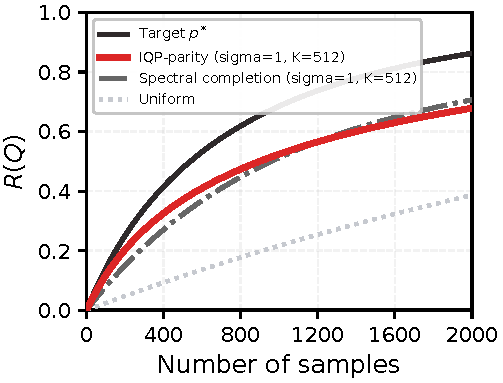
\includegraphics[width=0.32\textwidth]{plots/experiment_4_recovery_sigmak_triplet/experiment_4_recovery_best_iqp_vs_best_spectral.pdf}\hfill
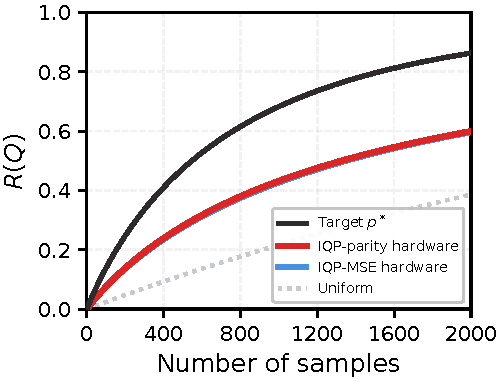
\includegraphics[width=0.32\textwidth]{plots/experiment_14_hardware_recovery_curve/experiment_14_hardware_recovery_curve_avg_common_seeds_hardware_only_no_spectral_paper.pdf}\hfill
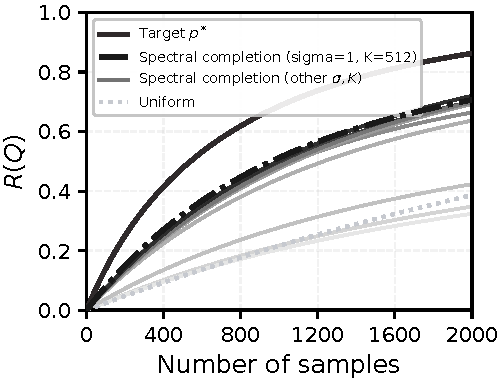
\includegraphics[width=0.32\textwidth]{plots/experiment_4_recovery_sigmak_triplet/experiment_4_recovery_spectral_sigmak_only.pdf}

\vspace{2pt}

{\footnotesize
(a) IQP vs.\ matched spectral proxy \hfill
(b) Global-best parity $(\sigma,K)=(1,512)$ vs.\ IQP-MSE on hardware \hfill
(c) Spectral family over $(\sigma,K)$
}

\caption{Mechanism at the representative fixed-$\beta$ point $\beta=0.9$. Panels (a) and (c) retain the simulation-side mechanism view. Panel (b) shows the corresponding hardware validation for the globally chosen parity setting $(\sigma,K)=(1,512)$ against IQP-MSE. The cumulative recovery curves $R_q(Q)$ provide a monotone view of the same finite-budget coverage process used in the high-value-state coverage analysis. The spectral curve is diagnostic only (cf.\ Sec.~\ref{sec:method:spectral}).}
\label{fig:spectral_mechanism}
\end{figure*}
